\scanpage{63}
\[
\chi_!(\widehat M^{\mathrm{an}}_{0,4})=\chi_!(\underbrace{U^{\mathrm{an}}_{0,3},\mathfrak S_4}_{-1/24})+\chi_!(\underbrace{\{0,1,\infty\},\mathfrak S_4}_{1/8})=\frac1{12}.
\]
De façon plus fine, dans un ``groupe de Grothendieck'' convenable, on aura
\margin{valable au dessus de $\mathbb Z[\frac16]$ --- \unsure{pour dispenser|pour me dispenser} de faire le calcul plus fin au dessus de $\operatorname{Spec}\mathbb Z\ldots$}
\[
79\quad\left\{\begin{aligned}
[M^!_{0,4}]&=[U_{\unsure{0,4|3,4}}]=\underbrace{T(1)}_{\substack{\text{``Tate''}\simeq[\mathbb E^1]\\(\text{d'augmentation }1)}}-2\\
[M_{0,4}]&=\deleted{\unsure{\tfrac1{24}(T(1)-2)}}\frac14(T(1)-2)+\frac1{12}+\frac18=\frac14(T(1)-1)-\frac1{24}\\
[\widehat M_{0,4}]&=[M_{0,4}]+\frac18=\deleted{\unsure{\tfrac1{24}(T(1)+1)}}=\frac14(T(1)-1)+\frac1{12}
\end{aligned}\right.
\]
Ces trois quantités sont d'augmentation égale resp\textsuperscript{t} : $-1,-1/24,1/12$.

$2^\circ)$ \uline{Cas \unsure{de|des}} $\widehat M_{1,1}$.
\diagram{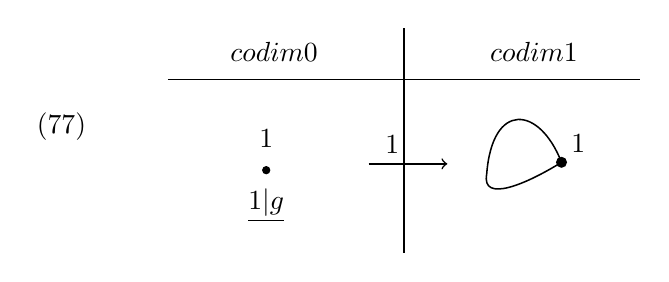
\begin{tikzpicture}[x=1cm,y=1cm,line width=.55pt]
\node at (-1.35,.55) {$(77)$};
\draw (0,1.15)--(6,1.15);
\draw (3,1.8)--(3,-1.05);
\node at (1.35,1.5) {$\text{codim }0$};
\node at (4.65,1.5) {$\text{codim }1$};
\fill (1.25,0) circle (1.5pt);
\node at (1.25,.4) {$1$};
\node at (1.25,-.45) {$\underline{\unsure{1|g}}$};
\draw[->] (2.55,.08)--(3.55,.08);
\node at (2.85,.32) {$1$};
\draw (5,.1)..controls(4.72,.82)and(4.12,.88)..(4.05,-.05)..controls(3.98,-.42)and(4.55,-.18)..(5,.1);
\fill (5,.1) circle (2pt);
\node[above right] at (5,.1) {$1$};
\end{tikzpicture}}
Il y a exactement un point à l'infini.

On a un morphisme (\uline{au dessus de} $\mathbb Z[\frac12]$)
\[
(78)\qquad \overset{\deleted{\unsure{\wedge}}}{M}_{1,1}\longrightarrow\overset{\deleted{\unsure{\wedge}}}{M}'_{1,4}\overset{\mathrm{déf}}{=}(\overset{\deleted{\unsure{\wedge}}}{M}^!_{1,4},\mathfrak S_3)
\]
qui fait de $\overset{\deleted{\unsure{\wedge}}}{M}_{1,1}$ une gerbe (de groupe constant $\{\pm1\}$) au dessus de $\overset{\deleted{\unsure{\wedge}}}{M}'_{1,4}$ (en ca. $\neq2$)
\[
\text{d'où}\qquad [M_{1,1}]=\frac12[U_{0,3},\mathfrak S_3]=\unsure{2|\frac12}[M_{0,4}]\underset{\inserted{T(1)}}{\deleted{\unsure{=\tfrac1{12}[\mathbb E^1]-\tfrac14}}}
\]
\margin{62}
